% This must be in the first 5 lines to tell arXiv to use pdfLaTeX, which is strongly recommended.
\pdfoutput=1
% In particular, the hyperref package requires pdfLaTeX in order to break URLs across lines.

\documentclass[11pt]{article}

% Remove the "review" option to generate the final version.
% \usepackage[review]{acl}
\usepackage{acl}

% Standard package includes
\usepackage{times}
\usepackage{latexsym}

% For proper rendering and hyphenation of words containing Latin characters (including in bib files)
\usepackage[T1]{fontenc}
% For Vietnamese characters
% \usepackage[T5]{fontenc}
% See https://www.latex-project.org/help/documentation/encguide.pdf for other character sets

% Typeset Chinese.
\usepackage{CJKutf8}
\newcommand{\SimCh}[1]{\begin{CJK}{UTF8}{gbsn}#1\end{CJK}}
\newcommand{\TraCh}[1]{\begin{CJK}{UTF8}{bsmi}#1\end{CJK}}

% This assumes your files are encoded as UTF8
\usepackage[utf8]{inputenc}

% This is not strictly necessary, and may be commented out,
% but it will improve the layout of the manuscript,
% and will typically save some space.
\usepackage{microtype}

% If the title and author information does not fit in the area allocated, uncomment the following
%
%\setlength\titlebox{<dim>}
%
% and set <dim> to something 5cm or larger.

\title{A Pratical way to perform Multi-Criteria Chinese Word Segmentation}

% Author information can be set in various styles:
% For several authors from the same institution:
% \author{Author 1 \and ... \and Author n \\
%         Address line \\ ... \\ Address line}
% if the names do not fit well on one line use
%         Author 1 \\ {\bf Author 2} \\ ... \\ {\bf Author n} \\
% For authors from different institutions:
% \author{Author 1 \\ Address line \\  ... \\ Address line
%         \And  ... \And
%         Author n \\ Address line \\ ... \\ Address line}
% To start a seperate ``row'' of authors use \AND, as in
% \author{Author 1 \\ Address line \\  ... \\ Address line
%         \AND
%         Author 2 \\ Address line \\ ... \\ Address line \And
%         Author 3 \\ Address line \\ ... \\ Address line}

\author{Tsu-Hsuan Chou \and Chun-Yi Lin \and Hung-Yu Kao \\
Intelligent Knowledge Management Lab \\
Institute of Computer Science and Information Engineering \\
National Cheng Kung University \\
Tainan, Taiwan \\
  \texttt{ProFatXuanAll@gmail.com}, \texttt{NE6101050@gs.ncku.edu.tw}, \\
  \texttt{hykao@mail.ncku.edu.tw}
}

% Utility commands.
\usepackage{mathtools}
\usepackage{multirow}
\usepackage{graphics}
\usepackage{stfloats}
\newcommand{\set}[1]{\lbrace #1 \rbrace}
\newcommand{\loss}{\mathcal{L}}
\newcommand{\CLS}{\texttt{[CLS]}}
\newcommand{\SEP}{\texttt{[SEP]}}
\newcommand{\UNC}{\texttt{[UNC]}}
\newcommand{\Ck}[1]{\texttt{[\(\mathtt{C}^{#1}\)]}}
\newcommand{\BTag}{\operatorname{B}}
\newcommand{\MTag}{\operatorname{M}}
\newcommand{\ETag}{\operatorname{E}}
\newcommand{\STag}{\operatorname{S}}
\newcommand{\TagSet}{\set{\BTag, \MTag, \ETag, \STag}}
\newcommand{\opClass}{\operatorname{class}}
\newcommand{\opCWS}{\operatorname{CWS}}
\newcommand{\opMCCWS}{\operatorname{MCCWS}}
\newcommand{\opFinal}{\operatorname{Final}}
\newcommand{\thetaC}{\theta_{\opClass}}
\DeclareMathOperator*{\argmax}{\arg\max}
\DeclarePairedDelimiter{\abs}{\lvert}{\rvert}

\begin{document}
\maketitle
\begin{abstract}
  Recent researches for multi-criteria Chinese word segmentation (MCCWS) are mainly focus on improving SOTA F1-score.
  Existing works always manually choose a suitable labeling criterion when perform training and evaluation, but fail to do so when perform inference, i.e., when suitable labeling criterion is unknown.
  Hence, to make MCCWS model a practical tool, one need to decide how to choose a suitable labeling criterion.
  In this work we show the need of additional criterion classification model and we proposed to use only one model to perform both word segmentation and choosing suitable labeling criterion.
  Experiments show that our MCCWS model has only minor F1-score degeneration (\(0.44\%\)) on average comparing to SOTA MCCWS model, meanwhile has the ability to choose criterion automatically and thus makes our MCCWS model practical.
  % Further analysis show that labeling inconsistency inside a dataset can be found by our method.
  Code to reproduce all experiments and details of all hyperparameters are available on GitHub \footnote{\url{http://acl-org.github.io/ACLPUB/formatting.html}}.
\end{abstract}

\section{Introduction}

In English, sentences are sequence of words with spaces in between.
This is not the case for some East-Asian languages like Chinese, Japanese or Korean, and it cause problems for one to process text in these languages.
Tokenizers for these languages, on the other hand, segment character sequences into smaller tokens, but may not respect the syntactic and semantic boundaries.
Thus, the need for Chinese word segmentation (CWS) tools is clear and CWS is still an on going research \citep{chen-etal-2017-adversarial,ma-etal-2018-state,He-2019-effective,Gong-2019-switch,huang-etal-2020-towards,huang-etal-2020-joint-multiple,ke2020unified,qiu-etal-2020-concise,ke-etal-2021-pre,tong-etal-2022-word}.

At present, \(97\%\) or higher F1-scores on CWS datasets are mainly achieved with single model per dataset.
But this means multiple model instances have to be saved and can cost a lot of spaces.
Therefore, it is ideal to use one model for all CWS datasets.
However, explicit degeneration has been observed when sharing one model across CWS datasets.
As point out first by \citep{chen-etal-2017-adversarial} and followed by many researches, the degeneration is mainly due to cross-dataset label inconsistency caused by different lingustic perspective.
For example, Chinese names, in their written form, do not have space between first name and last name, and some datasets segment last names while others do not.
For other example, consider idioms.
Frequently occured idioms are treated as single words.
But idioms frequently occured in one dataset may not frequently occured in others.
See Table~\ref{tab:label-inconsistency} for actual samples from datasets.

\begin{table}[t!]
  \centering
  \begin{tabular}{lll}
    \hline
    \textbf{Dataset} & \textbf{Samples}       & \textbf{Labels} \\
    \hline
    PKU              & \SimCh{江-泽民}        & S-BE            \\
    MSR              & \SimCh{江泽民}         & BME             \\
    \hline
    AS               & \TraCh{何-樂-而-不-為} & S-S-S-S-S       \\
    CIT              & \TraCh{何樂而不為}     & BMMME           \\
    \hline
  \end{tabular}
  \caption{Actual samples from different datasets \citep{emerson-2005-second} demonstrate labeling inconsistency.
    Hyphen ``-'' denotes segmentation.
    Labels are defined in Section~\ref{sec:data}.
    Last name \SimCh{江} is segmented in PKU dataset but no in MSR dataset.
    Idioms \TraCh{何樂而不為} is segmented in AS dataset but not in CIT dataset.
    Many more examples can be found in these datasets.
  }
  \label{tab:label-inconsistency}
\end{table}

Hence, to achieve higher F1-scores on CWS dataset with only one model, many researches proposed to used the so called multi-criteria learning on CWS model \citep{chen-etal-2017-adversarial,He-2019-effective,Gong-2019-switch,huang-etal-2020-towards,huang-etal-2020-joint-multiple,ke2020unified,qiu-etal-2020-concise,ke-etal-2021-pre}.
Here criteria (or criterion) means the labeling standard.
A multi-criteria CWS (MCCWS) model will receive both a character sequence and a criteria-specific hints to perform CWS.
In this way, we can train on much larger text corpus to make a CWS model more general, meanwhile have the ability to perform CWS with subtle differences.
Experiments show that MCCWS indeed perform better then CWS model without multi-criteria learning, and can achieve comparable performance compare to SOTA single model per dataset \citep{ke2020unified,ke-etal-2021-pre,tong-etal-2022-word}.

Despite the effectiveness of MCCWS model, one problem remains for MCCWS model to be practical.
When performing mulit-criteria learning on training sets or performing evaluation on test sets, one always know the pairing criterion for a given character sequence.
However, when performing inference, one do not know the pairing criterion in advanced.
This is not a problem when one know how to choose a criterion for a given character sequence.
But this is a problem when one do not know how to choose a suitable criterion, especially for those without lingustic background.
Hence, to make MCCWS models practical, one need to provide a way to choose a suitable criterion for a given character sequence.

In this work, we proposed to jointly train an auxiliary text classification task together with multi-criteria learning.
Our MCCWS model can automatically choose a suitable criterion for a character sequence, meanwhile only sacrificing a little (\(0.44\%\)) F1-score performance on average.
%% TODO: add ablation description.

\section{Related Works}\label{sec:related}

Early works achieved \(95\%\) F1-score on SIGHAN bakeoff 2005 datasets \citep{emerson-2005-second}.
Those works used either uni-directional or bi-directional recurrent neural networks \citep{Schuster-1997-bidirectional,graves-2005-framewise}, with or without conditional random field \citep{chen-etal-2017-adversarial,ma-etal-2018-state,He-2019-effective}.
Features were in the style of lookup tables;
advanced features like syntactic structures are not used.
% This is because one have syntactic structure only after words are defined, which happens only after CWS is performed.
Due to the recent advancement of large pre-trained language models, F1-score on CWS is now up to \(97\%\) \citep{huang-etal-2020-towards,huang-etal-2020-joint-multiple,ke2020unified,qiu-etal-2020-concise,ke-etal-2021-pre,tong-etal-2022-word}.
% Our experiments showed that by fine-tuning BERT~\citep{devlin-etal-2019-bert} on single CWS dataset, \(97\%\) F1-score can be easily achieved.

% As their are multiple CWS datasets with different labeling criterion, many researches start to propose MCCWS models.
\citep{chen-etal-2017-adversarial} is the first to propose a MCCWS model with two sub-models, one is called shared model and the other is called private model.
The shared model is trained to share common knowledge across CWS datasets, while the private model is aimed to learn criteria-specific knowledge.
The shared model is trained under a adversarial setting, so that the criterion discriminator cannot reliably predict the criterion based on input sequence, thus failed to provide an automechanism for choosing suitable criterion.

Following \citep{chen-etal-2017-adversarial}, many different private models were proposed.
\citep{Gong-2019-switch} proposed switched-LSTMs which can dynamically route between multiple BiLSTMs to encode features, thus remove the need for creating different private models for each CWS dataset.
However, \citep{Gong-2019-switch} also removed the criterion classification task, so there is no way for switched-LSTMs to automatically choose a suitable criterion for the given sequence, and similarly for other MCCWS works with private model settings (\citep{huang-etal-2020-towards,qiu-etal-2020-concise}).

Instead of using more and more complex private models, some proposed to make criterion as part of input and thus reduced the overall model complexity.
\citep{He-2019-effective} proposed to add two artificial tokens which represent the labeling criterion, and put them at the begining and the end of input sentence, and then use BiLSTM to perform MCCWS.
\citep{huang-etal-2020-joint-multiple} do the same as \citep{He-2019-effective} but use Transformer encoder \citep{vaswani-2017-attention} instead of BiLSTM.
\citep{ke-etal-2021-pre} also use Transformer encoder, but only one artifical token are added at the begining of input sentence.
These works always manually assign criterion tokens, and therefore cannot choose a suitable criterion automatically.

In summary, previous researches on MCCWS either not provide a way to choose a criterion, or always manually choose a criterion.
In our work, we proposed a simple yet ellgant way to make our MCCWS model automatically choose a suitable criterion for the given character sequence.

\section{Methodology}

In this section we describe the detail of our MCCWS model and the mechanism to make our model capable of choosing criterion automatically.
We first give a formal definition of CWS (Section~\ref{sec:data} and Section~\ref{sec:cws}), and then we formally define MCCWS model (Section~\ref{sec:mccws}).
After that, we introduce a criterion classification model (Section~\ref{sec:class}) to help MCCWS choose criterion.
Finally, we show that we can jointly train one model instead of two to make our MCCWS model capable of choosing criterion automatically (Section~\ref{sec:auto}).

\subsection{CWS Dataset}\label{sec:data}

Let \(D\) be a CWS datasets.
Let \((x, y) \in D\) be a input-output pair sampled from \(D\).
\(x\) is a sequence of characters with length \(\abs{x}\), and we denote the \(i\)-th character of \(x\) as \(x_i\) where \(1 \leq i \leq \abs{x}\).
Each \(x_i\) will be assigned with a label \(y_i\) where \(y_i\) is the \(i\)-th element of \(y\).
Hence, \(y\) is a sequence of labels with length equal to \(\abs{x}\).
Each \(y_i\) belongs to the tagset \(\TagSet\).
If \(y_i = \STag\), then \(x_i\) is itself a word, i.e., a word that is consist of single character \(x_i\).
If \(y_i \neq \STag\), then \(x_i\) is part of a word with at least \(2\) characters.
If \(x_i\) is in a word with exactly \(2\) characters, then \(y_i \in \set{\BTag, \ETag}\) where \(\BTag\) stands for ``the begining of a word'' and \(\ETag\) stands for ``the end of a word''.
If \(x_i\) is in a word with more than \(2\) characters, then \(y_i \in \set{\BTag, \MTag, \ETag}\) where \(\MTag\) stands for ``the middle of a word''.
See Table~\ref{tab:label-inconsistency} for examples.

\subsection{CWS Model}\label{sec:cws}

The goal of a CWS model with parameter \(\theta\) is to maximize the conditional probability \(\Pr(y | x ; \theta)\) for each \((x, y)\) in a CWS dataset \(D\).
The likelihood of each \((x, y) \in D\) is defined to be the product of the conditional probability of \(y_i\) given \(x\), i.e.,
\begin{equation}\label{eq:1}
  \Pr(y | x ; \theta) = \prod_{i = 1}^{\abs{x}} \Pr(y_i | x ; \theta).
\end{equation}
Let \(\abs{D}\) represent the number of \((x, y)\) pairs in the dataset \(D\).
To maximize the conditional probability \(\Pr(y | x ; \theta)\) with \(\theta\) for all \((x, y) \in D\), we can minimize the average negative log-likelihood of \(y\) given \(x\) over each \((x, y) \in D\):
\begin{equation}\label{eq:2}
  \loss_{\opCWS}(D ; \theta) = \dfrac{-1}{\abs{D}} \sum_{(x, y) \in D} \log \Pr(y|x ; \theta).
\end{equation}
We will revise Equations~\eqref{eq:1}\eqref{eq:2} to define a MCCWS model.

\subsection{MCCWS Model}\label{sec:mccws}

Let \(D^1, \dots, D^M\) be \(M\) different CWS datasets.
Each CWS dataset has its own labeling criterion, but all of them share the same tagset \(\TagSet\).
The goal of a MCCWS model is to train one CWS model on all \(M\) datasets at the same time and learn to perform CWS based on different labeling criterion.

Formally, given the \(m\)-th CWS dataset \(D^m\) and an input-output pair \((x, y) \in D^m\), a MCCWS model output the probability of \(y\) not just conditioning on \(x\) but also the labeling criterion \(C^m\) of \(D^m\).
Thus, we change Equation~\eqref{eq:1} to make the conditional probability also depends on \(C^m\):
\begin{equation}\label{eq:3}
  \Pr(y | x, C^m ; \theta) = \prod_{i = 1}^{\abs{x}} \Pr(y_i | x, C^m ; \theta)
\end{equation}
Now let \(D\) be the union of all datasets, i.e., \(D = \bigcup_{m = 1}^M D^m\).
Since we use \(M\) CWS datasets at the same time, we can treat \(M\) CWS dataset as one big CWS dataset \(D\) and minimize the average negative log-likelihood of \(y\) given \(x\) and the corresponding \(C^m\) of \(x\) over each \((x, y) \in D\).
So Equation~\eqref{eq:2} is changed into:
\begin{multline}\label{eq:4}
  \loss_{\opMCCWS}(D ; \theta) \\
  = \dfrac{-1}{\abs{D}} \sum_{m = 1}^M \sum_{(x, y) \in D^m} \log \Pr(y|x, C^m ; \theta).
\end{multline}
To perform inference, one need to give a MCCWS model both an input sequence \(x\) and a criterion \(C^m\), then one can use greedy decoding to get the prediction \(y\) given \(x\) and \(C^m\):
\begin{multline}\label{eq:5}
  y^* = \argmax_{y \in \TagSet^{\abs{x}}} \Pr(y | x, C^m ; \theta) \\
  = \argmax_{y_1, \dots, y_{\abs{x}} \in \TagSet} \prod_{i = 1}^{\abs{x}} \Pr(y_i | x, C^m ; \theta).
\end{multline}
The same optimization goal as in Equation~\eqref{eq:4} can be found in \citep{chen-etal-2017-adversarial,He-2019-effective,Gong-2019-switch,huang-etal-2020-towards,huang-etal-2020-joint-multiple,ke2020unified,qiu-etal-2020-concise,ke-etal-2021-pre}, and may written in the form of parameter \(\Theta^m\) when using private model or in the form of token \([m]\) when input together with character sequence (see Section~\ref{sec:related}).
As we will demonstrate in Section~\ref{sec:class}, using only Equation~\eqref{eq:4} to perform optimization cannot make a MCCWS model automatically choose a suitable labeling criterion for the given input \(x\), and thus make a MCCWS less practical.

\subsection{Auxiliary Classification Model}\label{sec:class}

From the formulation in Equations~\eqref{eq:3}\eqref{eq:4}\eqref{eq:5} we see that one have to give a MCCWS model both an input character sequence \(x\) and a labeling criterion \(C^m\).
Choosing criterion for training (see Equation~\eqref{eq:4}) is not a problem because every input-output pair must come from a CWS dataset \(D^m\) for some \(1 \leq m \leq M\).
And it is also not a problem for evaluation either (see Equation~\eqref{eq:5}), because we can assume the train-test split of a CWS dataset \(D^m\) have the same distribution.
It is a problem for inference (see Equation~\eqref{eq:5}), however, since one do not know which dataset the given input is coming from.
And it is this problem to make MCCWS almost practical.

If one always know which \(C^m\) to use for arbitrary character sequence \(x\), then the problem is solved.
Otherwise we need a tool to automatically choose \(C^m\) for a given \(x\).
One can do this by training a dataset classification model which models the probability of \(x\) coming from dataset \(D^m\) with parameter \(\thetaC\).
Again we use negative log-likelihood to optimize the dataset classification model:
\begin{multline}\label{eq:6}
  \loss_{\opClass}(D, \thetaC) \\
  = \dfrac{-1}{\abs{D}} \sum_{m = 1}^M \sum_{(x, y) \in D^m} \log \Pr(D^m | x ; \thetaC).
\end{multline}
After optimization, we can find the most possible dataset \(D^{m^*}\) for each character sequence \(x\) using our dataset classification model:
\begin{equation}\label{eq:7}
  m^* = \argmax_{1 \leq m \leq M} \Pr(D^m | x ; \thetaC).
\end{equation}
Then we use the corresponding criterion \(C^{m^*}\) to perform inference as in Equation~\eqref{eq:5}.
Thus, one need to train two models (one for MCCWS and one for dataset classification) to provide an automechanism for choosing suitable criterion.
In Section~\ref{sec:auto}, we proposed our MCCWS which can automatically choose criterion without auxiliary classification model.

We note that optimization goal similar to Equation~\eqref{eq:6} can be found in \citep{chen-etal-2017-adversarial}.
But they used adversarial training so that their auxiliary classification model can only provide nearly random prediction for dataset classification \citep{goodfellow-2014-gan}.
Besides, our average F1 performance is \(1.8\%\) higher comparing to \citep{chen-etal-2017-adversarial}.

\subsection{Automatically Choosing Criterion}\label{sec:auto}

\begin{figure*}[t!]
  \center
  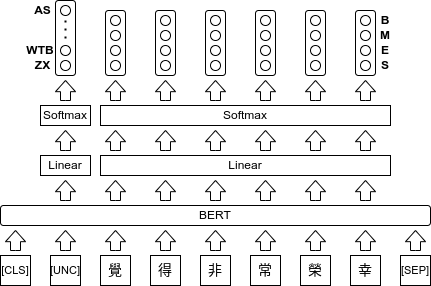
\includegraphics[width=.5\columnwidth]{./pic2.png}
  \caption{Our MCCWS model.
    Models will receive both criterion token and character sequence as input.
    The BERT encoder output are used to predict criterion and \(\TagSet\) for each position.
    Both \CLS{} and \SEP{} are added only because of implmentation details and we do no perform further computation on them.
    We add unknown criterion token \UNC{} to the input and perform \(M\)-way classification where \(M\) is the number of different CWS datasets.
    To manually choose a labeling criterion, one can replace \UNC{} with criteria-specific token \Ck{m} where \(1 \leq m \leq M\).}
  \label{fig:1}
\end{figure*}

Since \(D^m\) is built from some text corpus following the labeling criterion \(C^m\), we can assume that modeling \(x\) following labeling criterion \(C^m\) is equivalent to modeling \(x\) coming from dataset \(D^m\).
\begin{equation}\label{eq:8}
  \Pr(C^m | x ; \thetaC) = \Pr(D^m | x ; \thetaC).
\end{equation}
Now observe that
\begin{multline}\label{eq:9}
  \Pr(y | x, C^m ; \theta) \times \Pr(C^m | x ; \thetaC)                                                                              \\
  = \dfrac{\Pr(y, x, C^m ; \theta)}{\Pr(x, C^m ; \theta)} \times \dfrac{\Pr(x, C^m ; \thetaC)}{\Pr(x ; \thetaC)}.
\end{multline}
If we assume \(\thetaC = \theta\), then Equation~\eqref{eq:9} can be reduced to
\begin{equation}\label{eq:10}
  \dfrac{\Pr(y, x, C^m ; \theta)}{\Pr(x ; \theta)} = \Pr(y, C^m | x ; \theta).
\end{equation}
Hence, instead of optimizing two different models as in Equations~\eqref{eq:4}\eqref{eq:6}, we can optimize the joint probability of \(y\) and \(C^m\) given \(x\) with only one model \(\theta\).
This is equivalent to optimize the sum of Equations~\eqref{eq:4}\eqref{eq:6}:
\begin{multline}\label{eq:11}
  \loss_{\opFinal}(D ; \theta) = \loss_{\opMCCWS}(D ; \theta) + \loss_{\opClass}(D, \theta) \\
  = \dfrac{-1}{\abs{D}} \sum_{m = 1}^M \sum_{(x, y) \in D^m} \log \Pr(y, C^m | x ; \theta).
\end{multline}
Equation~\eqref{eq:11} is the keystone to make our MCCWS model capable of automatically choosing a suitable criterion for a given input.

In practice, we use BERT~\citep{devlin-etal-2019-bert} as our MCCWS model \(\theta\) (see Figure~\ref{fig:1}).
We define criteria-specific token \Ck{m} for each CWS dataset \(D^m\).
We define another token \UNC which represents ``unknown criterion''.
Each character sequence \(x\) is now paired with either its corresponding \Ck{m} or \UNC, but not both.
The new sequence is then input to BERT (only one \(\theta\) is used).
The BERT output of \(x\) is used to perform CWS.
The BERT output of the paired token is used to perform criterion classification.
If the paired token is \UNC, then perform criterion classification is equivalent to Equation~\eqref{eq:6}.
If the paired token is \Ck{m}, then perform criterion classification is equivalent to identity mapping, and perform CWS is equivalent to perform MCCWS as in Equation~\eqref{eq:4}.
Under our setting, our MCCWS model can automatically choose a suitable criterion for the given input, meanwhile have the option to manually choose labeling criterion by case.

% Our work in some way is similar to \citep{ke-etal-2021-pre}.
% We both use unknown criterion token \UNC and a criteria-specific token \Ck{m}.
% But they do so to perform meta-learning, and they never use \UNC to perform text classification and thus have no way to automatically choose a suitable criterion.
% While ours do not use meta-learning and we provide an auto mechanism to choose suitable labeling criterion.

\section{Experiments}

\begin{table}[t]
  \caption{Dataset statistics for training, development and test sets.}
  \label{tab:dset-stats}
  \centering
  \resizebox{1\columnwidth}{!}{
    \begin{tabular}{lccc}
      \textbf{Corpus} & \textbf{\#Train Words} & \textbf{\#Dev Words} & \textbf{\#Test Words} \\
      \hline
      AS              & 4.9M                   & 546K                 & 122K                  \\
      CITYU           & 1.3M                   & 146K                 & 40K                   \\
      CNC             & 5.8M                   & 727K                 & 726K                  \\
      MSRA            & 2.1M                   & 234K                 & 106K                  \\
      PKU             & 999K                   & 110K                 & 104K                  \\
      \hline
    \end{tabular}
  }
\end{table}

% \begin{table}[ht]
%   \caption{Dataset statistics for training, development and test sets.}
%   \label{tab:dset-stats}
%   \centering
%   % \resizebox{1\columnwidth}{!}{
%   \begin{tabular}{lccc}
%     \textbf{Corpus} & \textbf{\#Words in Train} & \textbf{\#Words in Dev} & \textbf{\#Words in Test} \\
%     \hline
%     AS              & 4.9M                      & 546K                    & 122K                     \\
%     CITYU           & 1.3M                      & 146K                    & 40K                      \\
%     CNC             & 5.8M                      & 727K                    & 726K                     \\
%     CTB6            & 678K                      & 51K                     & 52K                      \\
%     MSRA            & 2.1M                      & 234K                    & 106K                     \\
%     PKU             & 999K                      & 110K                    & 104K                     \\
%     SXU             & 475K                      & 52K                     & 113K                     \\
%     UD              & 98K                       & 12K                     & 12K                      \\
%     WTB             & 14K                       & 1K                      & 1K                       \\
%     ZX              & 67K                       & 20K                     & 67K                      \\
%     \hline
%   \end{tabular}
%   % }
% \end{table}

\subsection{Datasets and Experiments Setup}\label{sec:hps}

We use five publicly available CWS datasets, one is CNC\footnote{\url{http://corpus.zhonghuayuwen.org/}} and the others are from SIGHAN2005 bakeoff \cite{emerson-2005-second}, including AS, CITYU, PKU and MSRA.
Only AS and CITYU are in traditional Chinese, the rest are in simplified Chinese.
For CNC, we use the official split of train, development and test sets.
For AS, CITYU, MSRA and PKU, we randomly pick \(10\%\) of data from training set as development set.
Following \cite{cai-etal-2017-fast}, we first convert full-width characters into half-width characters, then we convert consecutive digits and english characters into single token, while respecting spaces if there is any.
No conversion is made between traditional and simplified Chinese.
On training set sentences are set to have at most \(512\) characters.
On validation and test sets sentences are splited as training and then merge back to their original form after inference.
Dataset statistics can be found in Table~\ref{tab:dset-stats}.

% We use four publicly available CWS datasets from SIGHAN2005 bakeoff \cite{emerson-2005-second}, including AS, CITYU, PKU and MSRA.
% Unfortunately, we are not able to access datasets from SIGHAN2008 bakeoff \cite{jin-chen-2008-fourth} since their website is currently down.
% We instead use another four publicly available datasets, including CNC\footnote{\url{http://corpus.zhonghuayuwen.org/}}, CTB6 \cite{xue-2015-ctb}, UD \cite{zeman-etal-2018-conll} and ZX \cite{zhang-etal-2014-type}.
% We use eight datasets in total (\(M = 8\)).
% We instead use another five publicly available datasets, including CNC\footnote{\url{http://corpus.zhonghuayuwen.org/}}, CTB6 \cite{xue-2015-ctb}, UD \cite{zeman-etal-2018-conll}, WTB \cite{wang-etal-2014-dependency} and ZX \cite{zhang-etal-2014-type}.
% We use \(10\) datasets in total (\(M = 10\)).

% For CNC, CTB6, UD and ZX, we use the official split of train, development and test sets.
% For AS, CITYU, MSRA and PKU, we randomly pick \(10\%\) of data from training set as development set.
% Following \cite{cai-etal-2017-fast}, we convert consecutive digits and english characters into single token, while respecting spaces if there is any.
% We convert full-width characters into half-width characters.
% No conversion is made for traditional and simplified Chinese.
% On training set sentences are set to have maximum characters \(64\).
% On validation and test sets sentences are splited as training and then merge back to their original form after inference.
% Dataset statistics can be found in Table~\ref{tab:dset-stats}.
% For CNC, CTB6, UD, WTB and ZX, we use the official split of train, development and test sets.
% For AS, CITYU, MSRA and PKU, we randomly pick \(10\%\) of data from training set as development set.
% Following \cite{cai-etal-2017-fast}, we convert consecutive digits and english characters into single token, while respecting spaces if there are any.
% We convert full-width characters into half-width characters.
% No conversion is made for traditional and simplified Chinese.
% Dataset statistics can be found in Table~\ref{tab:dset-stats}.

We use Pytorch \cite{paszke-etal-2019-pytorch} to implement our model.
We fine-tune BERT with AdamW \cite{loshchilov2018decoupled} on the pre-trained checkpoint \texttt{bert-base-case}\footnote{\url{https://huggingface.co/bert-base-chinese}} provided by hugginface \cite{wolf2019huggingface}.
Moving average coefficients \((\beta_1, \beta_2)\) of AdamW is set to \((0.9, 0.999)\).
Learning rate is set to \(2 \times 10^{-5}\) and weight decay coefficient is set to \(0.01\).
We schedule learning rate with linear warmup and linear decay.
Warmup ratio is set to \(0.1\).
We set batch size to \(32\) and we update our MCCWS \(250000\) times.
Then we pick the checkpoint with the highest F1 on development set to calculate test set F1.

Each sample in a CWS dataset is paired with corresponding criteria-specific token \Ck{m}.
We randomly replace \(50\%\) of \Ck{m} with \UNC.
As in \cite{devlin-etal-2019-bert}, we added two linear layer with softmax on top of the BERT encoder output, one for computing \(\Pr(C^k | x ; \theta)\) and one for computing \(\Pr(y | x, C^k ; \theta)\).
See Figure~\ref{fig:1} for model architecture.

\subsection{Overall Results}

\begin{table*}[t]
  \caption{F1-score (in percentage) on all five CWS datasets.
    F1-scores other than ours are directly recorded from their papers.
    \dag: Manually choosing criterion-specific token for each input.
    \ddag: Automatically choosing criterion for each input by giving \UNC.
  }
  \label{tab:f1}
  \centering
  % \resizebox{1\columnwidth}{!}{
  \begin{tabular}{lcccccccc}
    \hline
    \textbf{MCCWS Models}                                    & \textbf{AS}    & \textbf{CITYU} & \textbf{CNC}  & \textbf{MSRA} & \textbf{PKU}  & \textbf{Avg.}  \\
    \hline
    Model-I+ADV \cite{chen-etal-2017-adversarial}            & 94.64          & 95.55          & -             & 96.04         & 94.32         & 95.35          \\
    \cite{He-2019-effective}                                 & 95.47          & 95.60          & -             & 97.35         & 95.78         & 96.01          \\
    \cite{huang-etal-2020-joint-multiple}                    & -              & -              & 97.19         & 98.29         & 96.85         & -              \\
    \cite{huang-etal-2020-towards}                           & 97.0           & 97.8           & \textbf{97.3} & \textbf{98.5} & \textbf{97.3} & \textbf{97.68} \\
    Unified Transformer Encoder \cite{qiu-etal-2020-concise} & 96.44          & 96.91          & -             & 98.05         & 96.41         & 96.96          \\
    M{\small ETA}S{\small EG} \cite{ke-etal-2021-pre}        & \textbf{97.04} & \textbf{98.12} & 97.25         & 98.02         & 96.76         & 97.56          \\
    \hline
    \dag Ours                                                & 96.60          & 97.85          & 97.29         & 97.92         & 96.84         & 97.30          \\
    \ddag Ours + \UNC                                        & 96.55          & 97.71          & 96.91         & 95.33         & 95.26         & 96.35          \\
    \hline
  \end{tabular}
  % }
\end{table*}

% \begin{table*}[ht]
%   \caption{F1-score (in percentage) on all eight CWS datasets.
%     F1-scores other than ours are directly recorded from their papers.
%     Since not all researches use the same CWS datasets, we only report the average F1-score on five commonly used CWS datasets for fare comparison.
%     Five datasets include AS, CITYU, CTB6, MSRA and PKU.
%     \dag: Manually choosing criterion-specific token for each input.
%     \ddag: Automatically choosing criterion for each input by giving \UNC.
%   }
%   \label{tab:f1}
%   \centering
%   \resizebox{1\columnwidth}{!}{
%     \begin{tabular}{lccccccccc}
%       \hline
%       \textbf{MCCWS Models}                                    & \textbf{AS}    & \textbf{CITYU} & \textbf{CNC}  & \textbf{CTB6}  & \textbf{MSRA} & \textbf{PKU}  & \textbf{UD}    & \textbf{ZX}   & \textbf{avg. in 5} \\
%       \hline
%       Model-I+ADV \cite{chen-etal-2017-adversarial}            & 94.64          & 95.55          & -             & 96.18          & 96.04         & 94.32         & -              & -             & 95.35              \\
%       \cite{He-2019-effective}                                 & 95.47          & 95.60          & -             & 95.84          & 97.35         & 95.78         & -              & -             & 96.01              \\
%       \cite{huang-etal-2020-joint-multiple}                    & -              & -              & 97.19         & 97.56          & 98.29         & 96.85         & 97.69          & -             & -                  \\
%       \cite{huang-etal-2020-towards}                           & 97.0           & 97.8           & \textbf{97.3} & 97.8           & \textbf{98.5} & \textbf{97.3} & 97.8           & \textbf{97.1} & \textbf{97.68}     \\
%       Unified Transformer Encoder \cite{qiu-etal-2020-concise} & 96.44          & 96.91          & -             & 96.99          & 98.05         & 96.41         & -              & -             & 96.96              \\
%       M{\small ETA}S{\small EG} \cite{ke-etal-2021-pre}        & \textbf{97.04} & \textbf{98.12} & 97.25         & \textbf{97.87} & 98.02         & 96.76         & 83.84          & 88.48         & 97.56              \\
%       \hline
%       \dag Ours                                                & 96.61          & 97.77          & 97.07         & 97.62          & 97.54         & 96.65         & \textbf{97.86} & 96.87         & 97.24              \\
%       \ddag Ours + \UNC                                        & 96.56          & 97.28          & 96.67         & 96.92          & 94.45         & 95.44         & 97.33          & 96.23         & 96.13              \\
%       \hline
%     \end{tabular}
%   }
% \end{table*}

% \begin{table*}[ht]
%   \centering
%   \resizebox{2\columnwidth}{!}{
%     \begin{tabular}{lccccccccccc}
%       \hline
%       \textbf{Models}                                           & \textbf{AS} & \textbf{CITYU} & \textbf{CNC} & \textbf{CTB6} & \textbf{MSRA} & \textbf{PKU} & \textbf{SXU} & \textbf{UD} & \textbf{WTB} & \textbf{ZX} & \textbf{avg.} \\
%       \hline
%       Model-I+ADV \cite{chen-etal-2017-adversarial}            & 94.64       & 95.55          & -            & 96.18         & 96.04         & 94.32        & 96.04        & -           & -            & -           & 9             \\
%       Model-II+ADV \cite{chen-etal-2017-adversarial}           & 94.75       & 95.50          & -            & 96.0          & 95.94         & 94.13        & 95.96        & -           & -            & -           & 9             \\
%       Model-III+ADV \cite{chen-etal-2017-adversarial}          & 94.68       & 94.07          & -            & 96.1          & 95.87         & 94.25        & 96.14        & -           & -            & -           & 9             \\
%       \cite{He-2019-effective}                                 & 95.47       & 95.60          & -            & 95.84         & 97.35         & 95.78        & 96.49        & -           & -            & -           & 9             \\
%       \cite{huang-etal-2020-joint-multiple}                    & -           & -              & 97.19        & 97.56         & 98.29         & 96.85        & 97.56        & 97.69       & -            & -           & 9             \\
%       \cite{huang-etal-2020-towards}                           & 97.0        & 97.8           & 97.3         & 97.8          & 98.5          & 97.3         & 97.5         & 97.8        & 93.2         & 97.1        & 9             \\
%       Unified Transformer Encoder \cite{qiu-etal-2020-concise} & 96.44       & 96.91          & -            & 96.99         & 98.05         & 96.41        & 97.61        & -           & -            & -           & 9             \\
%       M{\small ETA}S{\small EG} (w/o finte-tune)                & 97.04       & 98.12          & 97.25        & 97.87         & 98.02         & 96.76        & 97.51        & 83.84       & 89.53        & 88.48       & 9             \\
%       M{\small ETA}S{\small EG}                                 & 97.01       & 98.20          & 97.55        & 97.89         & 98.50         & 96.92        & 97.88        & 98.57       & 93.97        & 97.22       & 9             \\
%       \hline
%     \end{tabular}
%   }
%   \caption{caption}
%   \label{tab:f1}
% \end{table*}

Table~\ref{tab:f1} shows the results of our experiments.
Our MCCWS achieved \(97.24\%\) on average F1-score over five CWS datasets, which is only \(0.44\%\) less comparing to SOTA MCCWS model.
We note that our MCCWS model is far simpler comparing to others, since we don't use CRF layer and any other handcrafted features.
% If we instead average F1-scores over all eights datasets, then our MCCWS achieved \(97.24\%\) and SOTA achieved \(97.57\%\), which makes our gap even smaller.
% This suggests our MCCWS model does not suffer from serious degeneration when jointly trained to perform criterion classification.

To demonstrate the ability of automatically choosing suitable criterion for each character sequence, we give our MCCWS model \UNC{} to perform inference.
Table~\ref{tab:f1} shows that under this setting we can achieve \(96.13\%\) F1-score on average which is only \(1.54\%\) less compare to SOTA MCCWS model.
This suggests our MCCWS model is indeed a practical tool.

\subsection{Ablation Study}

\begin{table*}[t]
  \caption{UNC prediction accuracy.}
  \label{tab:acc}
  \centering
  % \resizebox{.7\columnwidth}{!}{
  \begin{tabular}{lccccccc}
    \hline
                   & \textbf{AS} & \textbf{CITYU} & \textbf{CNC} & \textbf{MSRA} & \textbf{PKU} \\
    \hline
    \textbf{AS}    & 99.27       & 5.69           & 0.18         & 0.40          & 0.05         \\
    \textbf{CITYU} & 0.69        & 94.17          & 0.01         & 0.05          & 0.15         \\
    \textbf{CNC}   & 0.0         & 0.0            & 94.29        & 27.55         & 8.78         \\
    \textbf{MSRA}  & 0.0         & 0.0            & 5.41         & 63.09         & 21.29        \\
    \textbf{PKU}   & 0.03        & 0.13           & 0.12         & 8.91          & 69.73        \\
    \hline
  \end{tabular}
  % }
\end{table*}

\begin{table*}[t]
  \caption{Wrong token inference F1.}
  \label{tab:tkinf}
  \centering
  % \resizebox{.7\columnwidth}{!}{
  \begin{tabular}{lccccccc}
    \hline
                   & \textbf{AS} & \textbf{CITYU} & \textbf{CNC} & \textbf{MSRA} & \textbf{PKU} \\
    \hline
    \textbf{AS}    & 96.60       & 97.17          & 96.95        & 95.08         & 95.22        \\
    \textbf{CITYU} & 95.54       & 97.85          & 96.07        & 96.60         & 94.95        \\
    \textbf{CNC}   & 96.51       & 97.67          & 97.29        & 90.85         & 95.25        \\
    \textbf{MSRA}  & 95.92       & 97.15          & 94.06        & 97.92         & 94.42        \\
    \textbf{PKU}   & 95.63       & 97.07          & 92.78        & 87.80         & 96.84        \\
    \hline
  \end{tabular}
  % }
\end{table*}

Table~\ref{tab:acc} show our criterion prediction accuracy.

% Some intro to CWS.
% (1) necessity for CWS.
% (2) distinction from tokenization.
% (3) simple comparison for CWS and BPE.
% (4) recent work using pre-train model.
% Some intro to Multi-CWS.
% (1) giving examples.
% (2) emphasize pros, including memory size, easily change criterion
% (3) emphasize cons, one have to choose criterion manually, this is a problem when you don't know lingustic, our goal is to solve it.
% Specify our task and model definition
% (1) which dataset, is it open or closed
% (2) which model, algorithm and hyperparameters.
% (3) optimization process and hyperparameters.
% Notes
% (1) point out the similarity of between us and \citep{ke-etal-2021-pre}.

% These instructions are for authors submitting papers to *ACL conferences using \LaTeX.
% They are not self-contained.
% All authors must follow the general instructions for *ACL proceedings,\footnote{\url{http://acl-org.github.io/ACLPUB/formatting.html}} and this document contains additional instructions for the \LaTeX{} style files.

% The templates include the \LaTeX{} source of this document (\texttt{acl.tex}),
% the \LaTeX{} style file used to format it (\texttt{acl.sty}),
% an ACL bibliography style (\texttt{acl\_natbib.bst}),
% an example bibliography (\texttt{custom.bib}),
% and the bibliography for the ACL Anthology (\texttt{anthology.bib}).

% \section{Engines}

% To produce a PDF file, pdf\LaTeX{} is strongly recommended (over original \LaTeX{} plus dvips+ps2pdf or dvipdf). Xe\LaTeX{} also produces PDF files, and is especially suitable for text in non-Latin scripts.

% \section{Preamble}

% The first line of the file must be
% \begin{quote}
%   \begin{verbatim}
% \documentclass[11pt]{article}
% \end{verbatim}
% \end{quote}

% To load the style file in the review version:
% \begin{quote}
%   \begin{verbatim}
% \usepackage[review]{acl}
% \end{verbatim}
% \end{quote}
% For the final version, omit the \verb|review| option:
% \begin{quote}
%   \begin{verbatim}
% \usepackage{acl}
% \end{verbatim}
% \end{quote}

% To use Times Roman, put the following in the preamble:
% \begin{quote}
%   \begin{verbatim}
% \usepackage{times}
% \end{verbatim}
% \end{quote}
% (Alternatives like txfonts or newtx are also acceptable.)

% Please see the \LaTeX{} source of this document for comments on other packages that may be useful.

% Set the title and author using \verb|\title| and \verb|\author|. Within the author list, format multiple authors using \verb|\and| and \verb|\And| and \verb|\AND|; please see the \LaTeX{} source for examples.

% By default, the box containing the title and author names is set to the minimum of 5 cm. If you need more space, include the following in the preamble:
% \begin{quote}
%   \begin{verbatim}
% \setlength\titlebox{<dim>}
% \end{verbatim}
% \end{quote}
% where \verb|<dim>| is replaced with a length. Do not set this length smaller than 5 cm.

% \section{Document Body}

% \subsection{Footnotes}

% Footnotes are inserted with the \verb|\footnote| command.\footnote{This is a footnote.}

% \subsection{Tables and figures}

% See Table~\ref{tab:accents} for an example of a table and its caption.
% \textbf{Do not override the default caption sizes.}

% \begin{table}
%   \centering
%   \begin{tabular}{lc}
%     \hline
%     \textbf{Command} & \textbf{Output} \\
%     \hline
%     \verb|{\"a}|     & {\"a}           \\
%     \verb|{\^e}|     & {\^e}           \\
%     \verb|{\`i}|     & {\`i}           \\
%     \verb|{\.I}|     & {\.I}           \\
%     \verb|{\o}|      & {\o}            \\
%     \verb|{\'u}|     & {\'u}           \\
%     \verb|{\aa}|     & {\aa}           \\\hline
%   \end{tabular}
%   \begin{tabular}{lc}
%     \hline
%     \textbf{Command} & \textbf{Output} \\
%     \hline
%     \verb|{\c c}|    & {\c c}          \\
%     \verb|{\u g}|    & {\u g}          \\
%     \verb|{\l}|      & {\l}            \\
%     \verb|{\~n}|     & {\~n}           \\
%     \verb|{\H o}|    & {\H o}          \\
%     \verb|{\v r}|    & {\v r}          \\
%     \verb|{\ss}|     & {\ss}           \\
%     \hline
%   \end{tabular}
%   \caption{Example commands for accented characters, to be used in, \emph{e.g.}, Bib\TeX{} entries.}
%   \label{tab:accents}
% \end{table}

% \subsection{Hyperlinks}

% Users of older versions of \LaTeX{} may encounter the following error during compilation:
% \begin{quote}
%   \tt\verb|\pdfendlink| ended up in different nesting level than \verb|\pdfstartlink|.
% \end{quote}
% This happens when pdf\LaTeX{} is used and a citation splits across a page boundary. The best way to fix this is to upgrade \LaTeX{} to 2018-12-01 or later.

% \subsection{Citations}

% \begin{table*}
%   \centering
%   \begin{tabular}{lll}
%     \hline
%     \textbf{Output}           & \textbf{natbib command} & \textbf{Old ACL-style command} \\
%     \hline
%     \citep{Gusfield:97}       & \verb|\citep|           & \verb|\cite|                   \\
%     \citealp{Gusfield:97}     & \verb|\citealp|         & no equivalent                  \\
%     \citet{Gusfield:97}       & \verb|\citet|           & \verb|\newcite|                \\
%     \citeyearpar{Gusfield:97} & \verb|\citeyearpar|     & \verb|\shortcite|              \\
%     \hline
%   \end{tabular}
%   \caption{\label{citation-guide}
%     Citation commands supported by the style file.
%     The style is based on the natbib package and supports all natbib citation commands.
%     It also supports commands defined in previous ACL style files for compatibility.
%   }
% \end{table*}

% Table~\ref{citation-guide} shows the syntax supported by the style files.
% We encourage you to use the natbib styles.
% You can use the command \verb|\citet| (cite in text) to get ``author (year)'' citations, like this citation to a paper by \citet{Gusfield:97}.
% You can use the command \verb|\citep| (cite in parentheses) to get ``(author, year)'' citations \citep{Gusfield:97}.
% You can use the command \verb|\citealp| (alternative cite without parentheses) to get ``author, year'' citations, which is useful for using citations within parentheses (e.g. \citealp{Gusfield:97}).

% \subsection{References}

% \nocite{Ando2005,andrew2007scalable,rasooli-tetrault-2015}

% The \LaTeX{} and Bib\TeX{} style files provided roughly follow the American Psychological Association format.
% If your own bib file is named \texttt{custom.bib}, then placing the following before any appendices in your \LaTeX{} file will generate the references section for you:
% \begin{quote}
%   \begin{verbatim}
% \bibliography{custom}
% \end{verbatim}
% \end{quote}

% You can obtain the complete ACL Anthology as a Bib\TeX{} file from \url{https://aclweb.org/anthology/anthology.bib.gz}.
% To include both the Anthology and your own .bib file, use the following instead of the above.
% \begin{quote}
%   \begin{verbatim}
% \bibliography{anthology,custom}
% \end{verbatim}
% \end{quote}

% Please see Section~\ref{sec:bibtex} for information on preparing Bib\TeX{} files.

% \subsection{Appendices}

% Use \verb|\appendix| before any appendix section to switch the section numbering over to letters. See Appendix~\ref{sec:appendix} for an example.

% \section{Bib\TeX{} Files}
% \label{sec:bibtex}

% Unicode cannot be used in Bib\TeX{} entries, and some ways of typing special characters can disrupt Bib\TeX's alphabetization. The recommended way of typing special characters is shown in Table~\ref{tab:accents}.

% Please ensure that Bib\TeX{} records contain DOIs or URLs when possible, and for all the ACL materials that you reference.
% Use the \verb|doi| field for DOIs and the \verb|url| field for URLs.
% If a Bib\TeX{} entry has a URL or DOI field, the paper title in the references section will appear as a hyperlink to the paper, using the hyperref \LaTeX{} package.

% \section*{Acknowledgements}

% This document has been adapted
% by Steven Bethard, Ryan Cotterell and Rui Yan
% from the instructions for earlier ACL and NAACL proceedings, including those for
% ACL 2019 by Douwe Kiela and Ivan Vuli\'{c},
% NAACL 2019 by Stephanie Lukin and Alla Roskovskaya,
% ACL 2018 by Shay Cohen, Kevin Gimpel, and Wei Lu,
% NAACL 2018 by Margaret Mitchell and Stephanie Lukin,
% Bib\TeX{} suggestions for (NA)ACL 2017/2018 from Jason Eisner,
% ACL 2017 by Dan Gildea and Min-Yen Kan,
% NAACL 2017 by Margaret Mitchell,
% ACL 2012 by Maggie Li and Michael White,
% ACL 2010 by Jing-Shin Chang and Philipp Koehn,
% ACL 2008 by Johanna D. Moore, Simone Teufel, James Allan, and Sadaoki Furui,
% ACL 2005 by Hwee Tou Ng and Kemal Oflazer,
% ACL 2002 by Eugene Charniak and Dekang Lin,
% and earlier ACL and EACL formats written by several people, including
% John Chen, Henry S. Thompson and Donald Walker.
% Additional elements were taken from the formatting instructions of the \emph{International Joint Conference on Artificial Intelligence} and the \emph{Conference on Computer Vision and Pattern Recognition}.

% Entries for the entire Anthology, followed by custom entries
\bibliography{anthology,custom}

% \appendix

% \section{Example Appendix}
% \label{sec:appendix}

% This is an appendix.

\end{document}
